\documentclass[11pt]{article}
\usepackage{fullpage}
\usepackage{graphicx}
\usepackage{subfigure}
\usepackage{comment}
\usepackage[square]{natbib}
\usepackage{hyperref}
\setcounter{secnumdepth}{4}
\usepackage{enumitem}
\usepackage{txfonts}
\usepackage{listings}
\lstset{breaklines=true}

\interfootnotelinepenalty=10000
\newcommand{\HRule}{\rule{\linewidth}{0.5mm}}

\hypersetup{ 			% parametrage des hyperliens
    colorlinks=true,	% colorise les liens
    breaklinks=true,	% permet les retours à la ligne pour les liens trop longs
    urlcolor= black,	% couleur des hyperliens
    linkcolor= black,	% couleur des liens internes aux documents (index, figures, tableaux, equations,...)
    citecolor= black	% couleur des liens vers les references bibliographiques
}

%numeroter les pages
\pagestyle{plain}


\begin{document}

\begin{titlepage}

\begin{center}

% Upper part of the page
 


\includegraphics[width=0.8\textwidth]{./header}\\[1cm]
\textsc{\Large Master Research Internship}
\vspace{1cm}


\includegraphics[height=0.1\textheight]{./logos/cerv_2}

\includegraphics[height=0.1\textheight]{./logos/teeside}

\includegraphics[height=0.1\textheight]{./logos/fiu}

\includegraphics[height=0.1\textheight]{./logos/CHRU_Brest}


  
\vspace{1cm} 
\textsc{\Large Master Thesis }\\[0.5cm]


% The title of your report
\HRule \\[0.4cm]
%{ \Large \bfseries Virtual Reality and Schizophrenia }\\[0.4cm]
%{ \bfseries Therapeutic game based on  narrative generation techniques }\\[0.2cm]
{ \Large \bfseries Therapeutic game based on }\\[0.4cm]
{ \Large \bfseries narrative generation techniques }\\[0.4cm]
{ \Large \bfseries for Schizophrenia }\\[0.2cm]
\HRule \\[1.5cm]
% The domain of your research 
\begin{flushleft}
\textbf{Domain : Human-Computer Interaction - Artificial Intelligence \\[1cm]}
\end{flushleft}

%Design of a therapeutic game based on narrative generation techniques targeting emotional cognitive deficits.
% Author and supervisor(s)
\begin{minipage}{0.4\textwidth}
\begin{flushleft} \large
\emph{Author:}\\
Cindy  \textsc{Even}
\end{flushleft}
\end{minipage}
\begin{minipage}{0.4\textwidth}
\begin{flushright} \large
\emph{Supervisors:} \\[2ex]
%
% name(s) of your supervisor(s)
Anne-Gwenn \textsc{Bosser } \\
C\'{e}dric \textsc{Buche } \\
% Name of your team
IHSEV - Lab-STICC - France\\[2ex]
Jo\~{a}o \textsc{F. Ferreira } \\
Digital Futures Institute - UK
\end{flushright}
\end{minipage}

\vfill


% INCLUDE HERE THE LOGO OF YOUR INSTITUTION
\begin{flushleft}

\includegraphics[width=0.2\textwidth]{./logos/enib}
\end{flushleft}
\end{center}
\end{titlepage}

%************************************************************%

\begin{abstract}
\thispagestyle{empty}
Patients suffering from schizophrenia and related illnesses have difficulties in social interactions. The impact of several kinds of interventions on social cognition has been studied recently and one of the best outcomes in this area is the social skills training. Serious games can be developed allowing the patients to train in a realistic and safe environment, in order to improve their social skills. In this study we tackled the problem of finding a narrative generation technique adapted to the underlying structure of dialogues that could be used for social skills training. The variability of the dialogue is particularly interesting from a therapeutic point of view as it is important to be able to provide alternatives, to cause patients to respond to unforeseen situations in a safe environment. We explored the use of linear logic applied to narrative generation to generate a dialogue that is conducted by an Embodied Conversational Agent (ECA). We propose in this report a method of modelling a dialogue that provides verbal and non-verbal informations needed to animate the ECA and that allows patients interactions. Schizophrenic patients often have difficulties to express their emotions which produce a difference between the facial expression they express and their actual emotional state. In order to make them aware and to teach them how to overcome these deficits, the ECA adapts its behaviour depending on the facial expression perceived using a facial emotion recognition system. 
\end{abstract}
\newpage
% compile twice to get the table of contents
\tableofcontents
\setcounter{page}{1} 
\newpage


%*****************************************************************%
\section{Introduction}
This master thesis showcases the work I undertook during my master research internship which was conducted at the CERV (Centre Europ\'{e}en de R\'{e}alit\'{e} Virtuelle) within the IHSEV team and in partnership with the hospital of Bohars which is part of the CHU of Brest, the University of Teeside (UK) and the University FIU of Miami (Florida, USA). \\

It combines the issues of interactive storytelling and serious games for therapeutic purposes. Patients suffering from schizophrenia and related illnesses often have difficulties with social interactions. The impact of several kinds of interventions on social cognition has been studied recently and one of the best outcomes in this area is social skills training.\\

The initial objective was to find a narrative generation technique adapted to the underlying structure of the scenarios for social skills training that would obtain a sufficient level of variability for use in a therapeutic purpose. To answer this question the plan was to develop a prototype serious game using a game engine.\\

After further discussion with the psychiatric team we realised that the scenarios they could provide us were more akin to dialogues. The problem now was finding a narrative generation technique adapted to the underlying structure of dialogues, that could be use in social skills training. To address this problem we will prototype a serious game using an Embodied Conversational Agent (ECA) with whom the patient can interact.\\

In section~\ref{sec: State of the art} we will discuss the state of the art of the three topics involved in this problem. First, we will present the specific problems faced by people with schizophrenia and see how a serious game could provide real support in their treatment. Then we will study the requirement to build an ECA with whom the patient can interact.  Finally, we will examine different techniques for Interactive Storytelling that could be used to allow variations within the generated dialogue. \\

In section~\ref{sec: Contribution} we start by explaining in detail the reasons why we had to adapt the question of this internship. Secondly we list the different elements needed for the suggested solution of this problem. We then describe the application and the different system used for the ECA and the generation of the dialogue. Finally we show in detail the execution of the application. \\

In section~\ref{sec: Evaluations} we present the plan for the evaluation of our system. It includes technical, acceptance and performance evaluations. \\

Lastly in section~\ref{sec: Conclusion and future work} we establish an overall review of the solution suggested and mention some possible improvements and future work.

%-----------------------------------------------------------------%
\newpage
\section{State of the art} \label{sec: State of the art}
\subsection{Context}
Schizophrenic patients have severe cognitive impairment and cognitive disorders that contribute as much, or even more than other symptoms in their mental disability \citep{Green96}. Social cognition is the set of skills specifically dedicated to our relationships with others, allowing the perception, the treatment and the interpretation of social signals. Eighty-five percent of patients with schizophrenia have cognitive disorders \citep{Vianin03}.\\

The cognitive disorders from which schizophrenic patients suffer contribute prominently to their difficulties in daily life, particularly from a social point of view \citep{Peneau15}. The usual treatments (including pharmacological or psychotherapeutic) have little impact on cognitive functioning. New therapeutic tools, so-called cognitive remediation, have been developed over the last twenty years making it possible to act on previously inaccessible disorders. The authors also mention that this is a complementary approach that should be used in conjunction with other techniques. Just as with drug and psychotherapeutic treatment, cognitive remediation makes sense in an integrative practice, centered on the person and his recovery.\\

Currently at the CHU doctors use the book written by \citeauthor{Liberman05} to train schizophrenia patients in social skills. In this book it is explained that one of the major reasons why patients with schizophrenia have difficulty meeting their needs and coping with everyday life lies in their inability to express themselves effectively to others. Even when the most recognizable symptoms of mental illness are controlled by medical treatment, patients' ability to communicate effectively remains diminished.
\subsubsection{Description of a social interaction}
In their book, \citeauthor{Liberman05} explain that Social interaction can be divided into three phases, each requiring a distinct set of skills:
\begin{itemize}
\item The first phase requires perception capabilities to capture and perceive the useful information in social situations. In order to respond correctly, it is necessary to identify people who are likely to interact, recognize their feelings and wishes, listen properly to what they say and understand their objectives.
\item The second phase uses development capabilities to choose the style and content of the response that would be the most appropriate.
\item The final phase of communication requires the use of correct verbal content in conjunction with the appropriate delivery. Choosing the right words is important but the way we talk is often equally, if not more important than what is said. We must choose the right non-verbal expressions such as facial expressions, gestures, posture and eye contact. Furthermore, paralinguistic practices including correct intensity of voice, fluency, speech rate and tone must be observed.
\end{itemize}
In schizophrenic patients, interpersonal communication problems may reflect deficits in one or more of these phases. Social skills training can provide a viable solution to these issues and can help patients to overcome their difficulties in daily life. 
\subsubsection{Social skills training}
\citeauthor{Liberman05} also explain that by teaching patients how to more effectively communicate their emotions and desires with others, can help them overcome the problems of everyday life. Training in social skills is the method by which we can teach patients how to extend their behavioural repertoires and succeed in social situations where they had hitherto failed.
In order for the training in social skills to be effective and successful, the following basic principles must be applied:
\begin{itemize}
\item The use of a model and its imitation : the patient can learn by observing a third party whose behaviour is appropriate.
\item Behavioural rehearsal : practice regularly through simulations and role-playing.
\item Social reinforcement : giving feedback, comments, and suggestions to improve.
\end{itemize} 
This manual \citep{Liberman05} has been designed for those who are involved in mental health and rehabilitation to acquire the techniques and procedures for social skills training so they can use it in the institution where they work. A controlled clinical research has shown that social skills training can be effective both to increase the social competence of patients and to reduce their vulnerability to psychiatric symptoms such as depression, delusions, hallucinations and impulse control problems.\\

In their clinical study, \citeauthor{Park11} compared social skills training using virtual reality role-playing to social skills training using traditional role-playing. They established that the virtual reality application was particularly beneficial in terms of improving conversational skills and assertiveness, concluding that it may be a useful supplement to traditional social skills training. 
\subsubsection{Benefits of serious games for health}
Engaging a patient's motivation is frequently necessary in health care because patients can be required to undergo procedures that are painful and aversive on the one hand, or boring and mundane on the other \citep{Kato12}.\\

\citeauthor{Kato12} explains that the repetitive nature of video game play is thought to be a key mechanism that promotes learning in games . The focus of attention on an engaging distraction is also thought to be a key factor \citep{Thompson10}, entertainment likely attracts and holds the player's attention on the video game, thereby facilitating player's exposure to behaviour change procedures. \\

Another asset for serious games is their ability to adapt to the player. \citeauthor{Fernandez12} used technologies such as emotional recognition to continuously track the emotional state of the player during the game. The game automatically responds in return by modifying the game play difficulty. \\

\citeauthor{Kim11} suggest that virtual reality systems could provide viable environments for individuals to interact with social avatars, it may be one of the most promising tools for assessing social skills because it minimizes bias resulting from traditional assessment methods. A strength of using virtual reality and virtual avatars for social skills training is that they provide a safe, harmless, and well-controlled environment in which to practice social interaction without the repercussions of emotional frustration and feeling of failure which could be expected in the real world.\\

Positive reinforcement is very important in social skills training \citep{Bellack04}. It refers to the positive consequences following a behaviour that increase the likelihood of that behaviour occurring again. A great advantage is that the application can provide instant feedback to the player with sound effects, graphics (see Figure \ref{Figure Feedback}) or directly via the characters of the game. \citeauthor{Bellack04} points out that feedback can enhance a sense of accomplishment and personal pride and a strict avoidance of put-downs or criticism make participation an enjoyable, non-threatening learning experience.\\

\citeauthor{Thompson10} shows the importance of debriefing after a session of game. It helps the player to make meaningful connections between the game experience and the real world, thereby enhancing transfer of knowledge and skills. Debriefing is typically conducted after game play by asking players to respond to a series of open-ended questions that explore their perceptions toward the game.\\

The use and participation of serious games are usually readily accepted by patients with mental disorders \citep{Fernandez12}. They have direct clinical implications because they can help improve patient participation in important diagnostic tasks, enhance knowledge about their disease, and increase patient adherence to aversive yet lifesaving treatments \citep{Kato12}.\\
\begin{figure}[!h]
   	\centerline{\includegraphics[scale=0.12]{./images/feedbacks}}
   	\caption{\label{Figure Feedback} Immediate Feedback by graphical effects \citep{Thompson10}}
\end{figure}

%-----------------------------------------------------------------%
\subsection{Social interaction with a Virtual Human}
The benefit of using virtual avatars for role playing training, comes from taking advantage of the fact that they can consistently present emotional stimuli at the will of the clinician \citep{Kim11}. Whereas the effectiveness of conventional role playing methods are often limited by the expressive capacity of the clinician/trainer. \\

It appears that schizophrenic patients exhibit a variety of deficits affecting emotion; they have not only a lesser expressiveness, making it difficult to communicate their own emotional state to others, but also a decreased ability to decode the emotional state of others through facial expression \citep{Peyroux14}.\\

Ga\"{i}a \citep{Gaudelus12} is a cognitive remediation program intended for people with schizophrenia or related disorders that have a reduced ability to recognise facial information. It takes place in four phases: emotion recognition on photos; followed by the same task using videos; role playing with the psychiatrist; and tasks to complete at home to promote the transfer of the strategies used during the session to daily life. This program is focused on increasing patients' ability to decode the emotional state of other but does not address the patients issues with expressing their emotions.\\

Patients also have a deficit in the recognition of their own expressions and are not aware of these difficulties. According to \citeauthor{Weiss09}, all these difficulties and the lack of their awareness could encourage the emergence of inappropriate social behaviour and could have important consequences on their relationships. It therefore appears important to develop cognitive remediation strategies focused on these deficits.\\

Embodied Conversational Agents (ECAs) are autonomous agents with a human-like appearance and communicative skills and they ought to be entities with dialogic and expressive capacities \citep{Pelachaud05}. To be involved in a communicative process the agent needs to perceive signs displayed buy the user and to emit signs.

\subsubsection{Existing Embodied Conversational Agents (ECAs)}
There are many ECA that have been successfully developed over the years using a large range of different input and generated output, here are few examples :\\

The agent Max \citep{Kopp05} is employed as a guide in a public computer museum. It engages with visitors in natural face-to-face communication, provides them with information about the museum or the exhibition, and conducts natural small talk conversations.\\

The agent Greta \citep{DeRosis03} is a real-time three dimensional embodied conversational agent with a 3D model of a woman compliant with MPEG-4 animation standard. It is able to communicate using a rich palette of verbal and nonverbal behaviours. It can talk and simultaneously show facial expressions, gestures, gaze, and head movements.\\

The Companions project has resulted in the development of a social agent,  which unlike the agent Max, focuses more on the relationship it can establish with the user than on the assistance or information it can provide for a particular task \citep{Smith11}. The second particularity of this system is that it manages user's interruptions. This system integrates 15 different software components covering the aspects of mutimodal affective input, affective dialogue processing, interruption management and mutlimodal affective output, which shows the complexity of such a system. Another originality of this system that is especially interesting in your problem is that, unlike the other ECAs described, it uses planning techniques for the generation of the ECA's narrative response.
\begin{figure}[!h]
   	\centerline{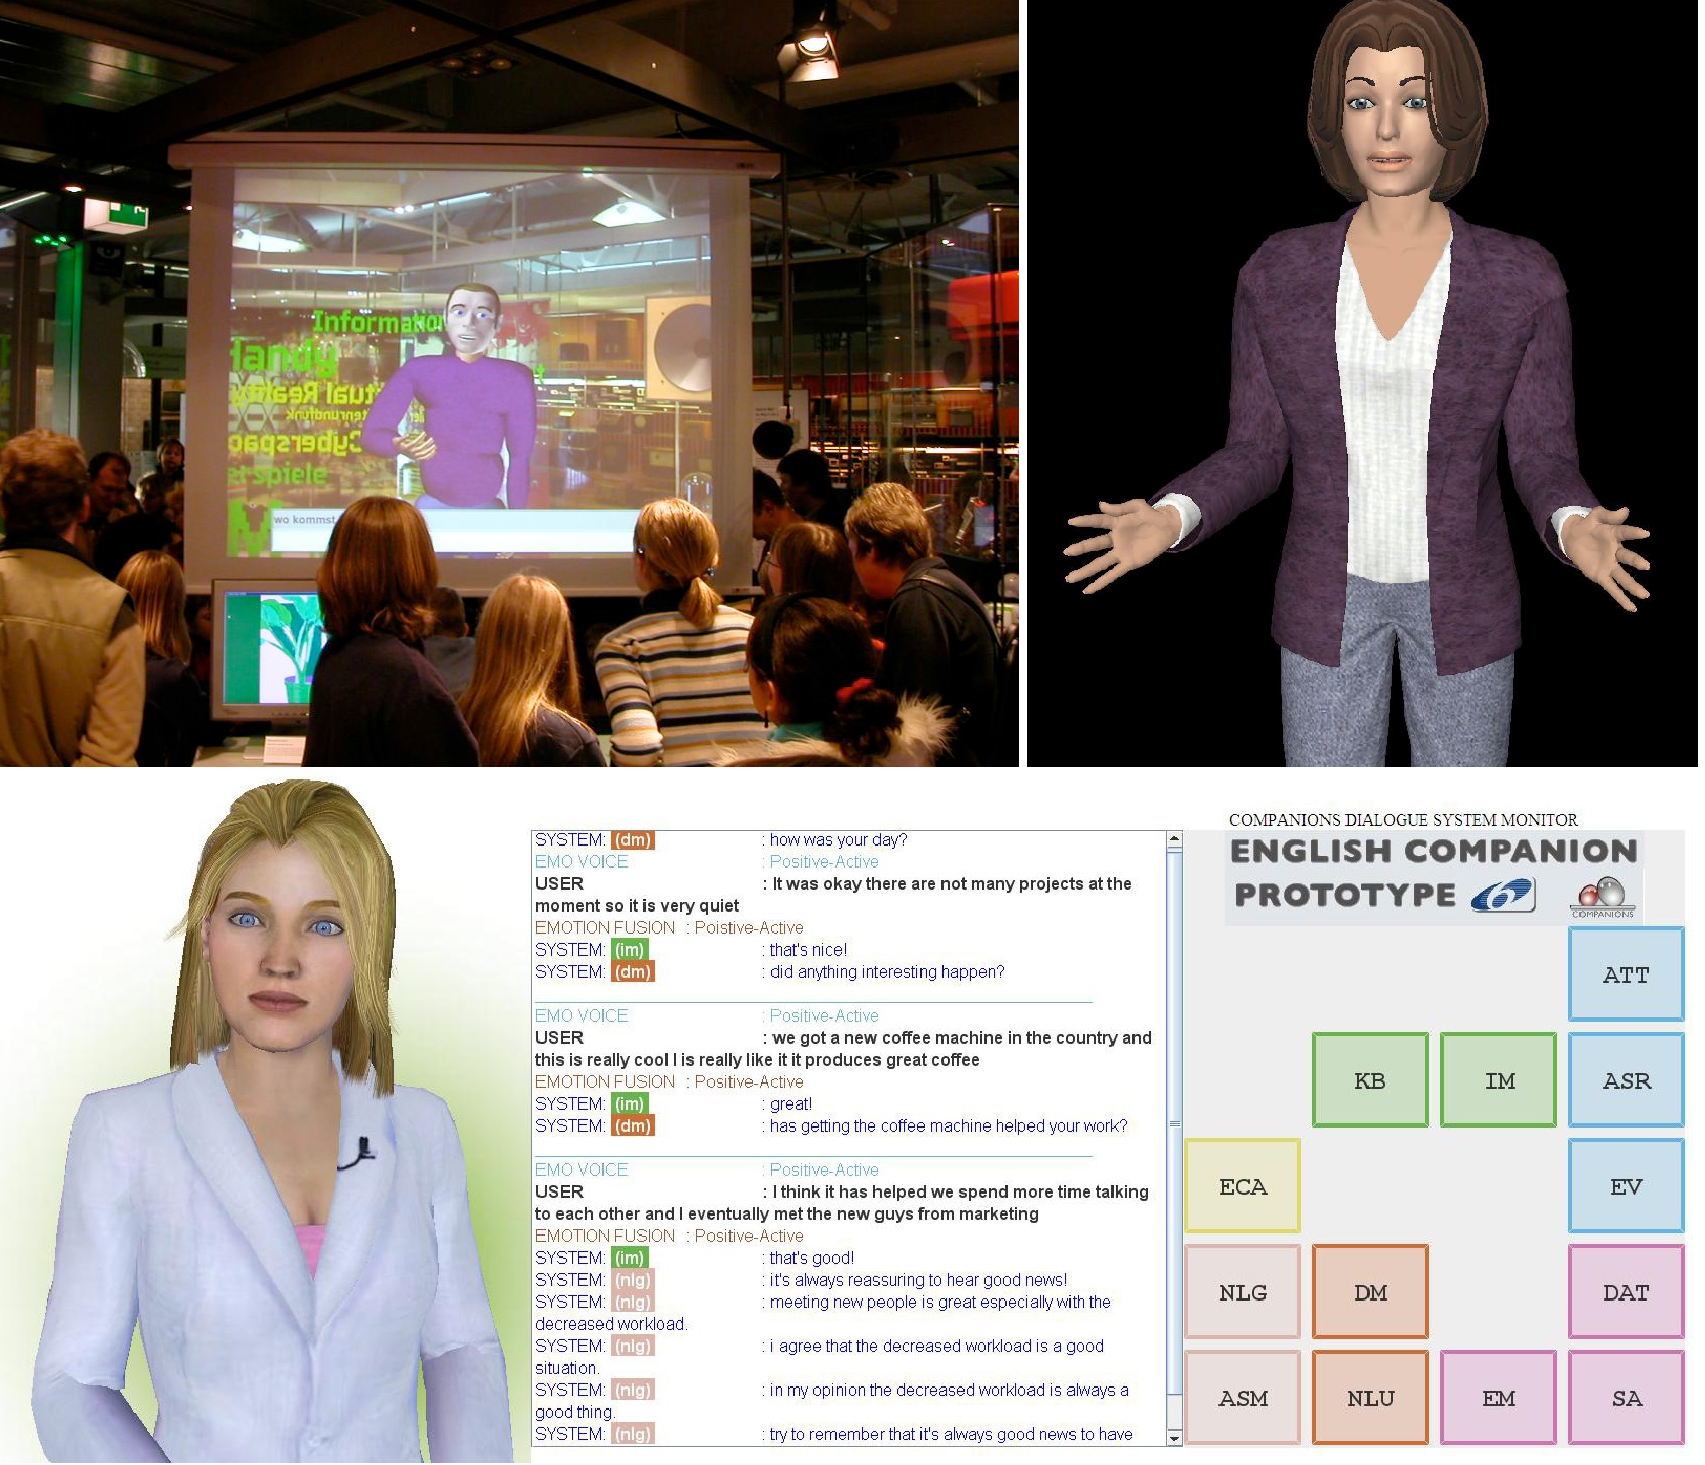
\includegraphics[scale=0.3]{./images/ECAs}}
   	\caption{\label{Figure ECAs} Top left : The agent Max interacting with visitors in the Heinz Nixdorf MuseumsForum \citep{Kopp05} | Top right : The agent Greta \citep{Pelachaud05} | Bottom : The English prototype for the Companions Project\citep{Smith11}}
\end{figure}
\subsubsection{Perception capabilities of ECAs}
To be able to adapt its behaviour, the ECA needs to perceive and pay attention to the users. This can be done using facial recognition for example. In the SimSensei Kiosk \citep{DeVault14} (a multimodal research platform for real-time assessment of distress indicators), the MultiSense framework was used (see Figure \ref{Figure visio}). The system automatically tracks and analyses in real-time facial expressions, body posture, acoustic features, linguistic patterns and higher-level behaviour descriptors (e.g. attention and fidgeting). These informative signals are broadcasted to another component of SimSensei Kiosk to inform the virtual human of the state and actions of the participant and assist with turn taking, listening feedback, and building rapport by providing appropriate non-verbal feedback. \\
\begin{figure}[h]
   	\centerline{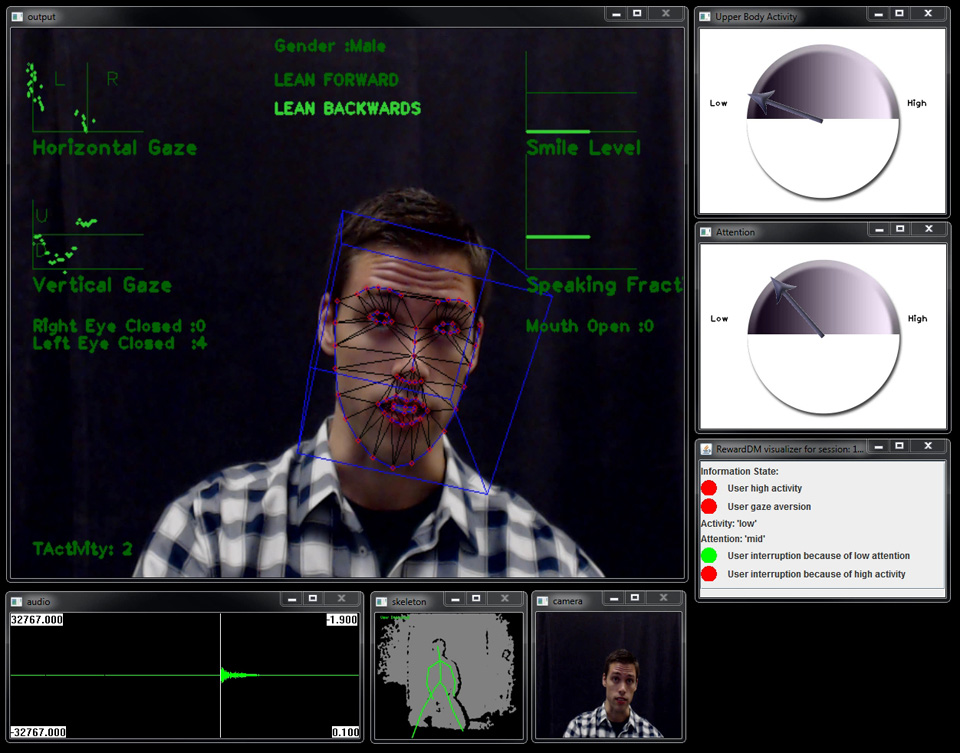
\includegraphics[scale=0.28]{./images/simsensei}}
   	\caption{\label{Figure visio} Multisense system \citep{DeVault14}}
\end{figure}

Speech emotion recognition can also be used. EmoVoice \citep{Vogt08} for example is a comprehensive framework for real-time recognition of emotions from acoustic properties of speech (which does not use word information) that can easily be plugged into other applications. This framework is widely used in research and appears in many applications such as Companions \citep{Smith11}, Greta \citep{DeRosis03} and in \citep{Pizzi11}.\\

The accuracy of these systems might be criticised \citep[see][p. 11]{Benyon13} but in their study, \citep{Busso04} show that the system based on facial expression give better performance than that based on just acoustic information for the emotions considered. Results also show that when these two modalities are fused, the performance and the robustness of the emotion recognition system improve measurably.\\

Another solution has been explored in the game PlayMancer \citep{Fernandez12}, a serious video game designed to remediate attitudinal, behavioural and emotional processes of patients with impulse-related disorders. \citeauthor{Fernandez12} used biosensors (based on the MobiHealth Mobile\textsuperscript{TM} system) to measure physiological signals such as galvanic skin response, oxygen saturation, heart rate (HR) and HR variation, skin temperature and breathing frequency and then extracted the emotional state of the user from these signals. The game automatically responds in return by modifying aspects of the game play difficulty. \\

Finally, psychological signals can be used for an electroencephalogram (EEG)-based emotion recognition. \citeauthor{Hamdi12} used this technology during his thesis \citep{Hamdi12} for an application to simulate job interviews. \\

In recent years, multimodal approach has become more and more common in emotional computing \citep{Hamdi12}. The objective is to record signals from various sensors and to implement mechanisms to jointly and effectively exploit the information gathered. The interest of the multimodal approach is the ability to improve the recognition of emotions and to reduce ambiguities that may arise when using a single signal.

\subsubsection{Generation of verbal and non-verbal behaviours}
To interact with the user, ECAs need to be able to give verbal and non-verbal messages. 
\paragraph{Facial expression}\mbox{}\\
The various facial behaviours and motions can be parametrised based on muscle actions. This set of parameters can then be used to represent the various facial expressions. To date, there have been two important and successful attempts in the creation of these parameter sets \citep{Bettadapura12}:
\begin{itemize}
\item The Facial Action Coding System (FACS) developed by Ekman and Friesen in 1977 \citep{Ekman77} and
\item The Facial Animation parameters (FAPs) which are a part of the MPEG-4 Synthetic/Natural Hybrid Coding (SNHC) standard, 1998 \citep{Pandzic03}.
\end{itemize}
\subparagraph{Facial Action Coding System (FACS)}
Facial Action Coding involves identifying the various facial muscles that individually or in groups cause changes in facial behaviours. These changes in the face or underlying (one or more) muscles are called Action Units (AU). \\

AUs can be additive or non-additive. AUs are said to be additive if the appearance of each AU is independent. Contrastly, AUs are said to be non-additive if they modify each other’s appearance. Having defined these, representation of facial expressions becomes an easy task. Each expression can be represented as a combination of one or more additive or non-additive AUs. For example ‘fear’ can be represented as a combination of AUs 1, 2 and 26. Figure \ref{Figure FACs} show some examples of upper face AUs and the facial movements that they produce when presented in combination.
\subparagraph{The Facial Animation Parameters (FAPs)}
The Moving Pictures Experts Group (MPEG) introduced the Facial Animation (FA) specifications in the MPEG-4 standard. Version 1 of the MPEG-4 standard became the international standard in 1999. It supports facial animation by providing Facial Animation Parameters (FAPs).\\

The MPEG-4 defines a face model in its neutral state to have a specific set of properties like a) all face muscles are relaxed; b) eyelids are tangent to the iris; c) pupil is 1/3rd the diameter of the iris and so on. Key features like eye separation, iris diameter, etc are defined on this neutral face model.\\

The standard also defines 84 key feature points (FPs) on the neutral face and the movement of the FPs is used to animate the faces. Figure \ref{Figure FAPs} shows the location of the 84 FPs on a neutral face as defined by the MPEG-4 standard.\\

68 FAPs are defined by the MPEG-4. They are a set of parameters that represent a complete set of facial actions along with head-motion, tongue, eye and mouth control. The FAP value indicates the magnitude of the FAP which in turn indicates the magnitude of the deformation that is caused on the neutral model.
\clearpage
\begin{figure}
   	\centerline{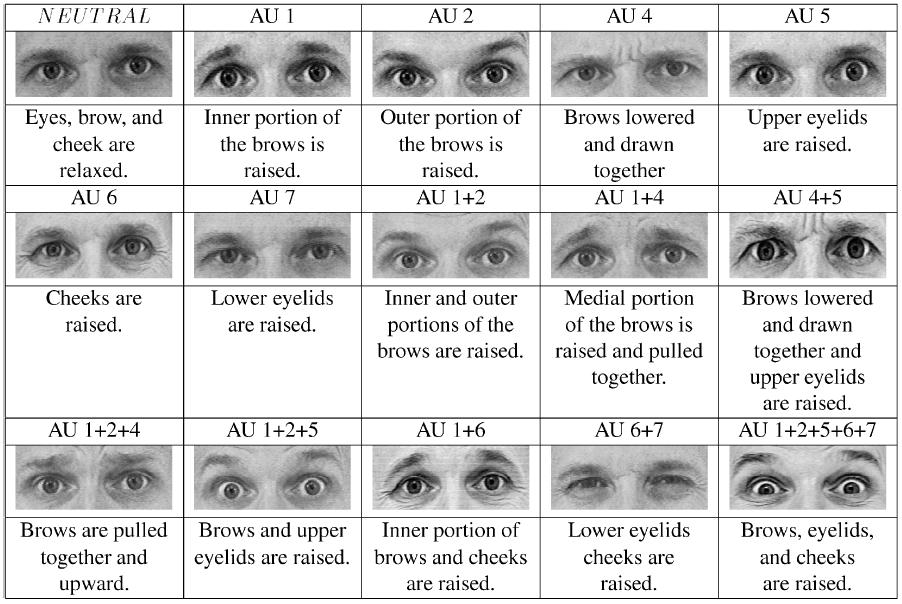
\includegraphics[scale=0.5]{./images/facs}}
   	\caption{\label{Figure FACs} Some of the upper face AUs and their combinations \citep{Tian01}}
\end{figure}
\begin{figure}
   	\centerline{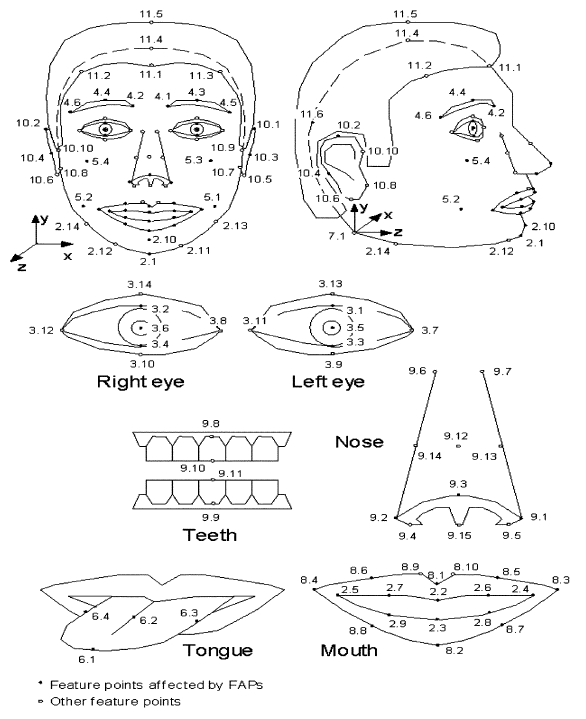
\includegraphics[scale=0.5]{./images/mpeg4}}
   	\caption{\label{Figure FAPs} The 84 Feature Points (FPs) defined on a neutral face \citep{Pandzic03}}
\end{figure}
\clearpage
\subparagraph{Duration of the expression}
In order for the ECA to be believable, the duration of the expression needs to be taken into account. In their study, \citeauthor{Verduyn09} show that the duration of emotional experience is highly variable. For example, the emotional episodes of fear are generally shorter than episodes of anger, which in turn are shorter than episodes of joy. They also identify a number of key predictors of the variability in the duration of emotional experience regardless of the exact nature of the emotion. These key predictors include the importance of the eliciting situation, the intensity of the emotion at onset, and reappearance (physical or mental) of the emotion-eliciting source.\\

To represent the temporal aspects of facial expressions, the agent Greta for example has its expressions characterized by four temporal parameters \citep{Pelachaud05}:
\begin{itemize}
\item Attack: time that the expression takes to reach its maximal intensity from the neutral face.
\item Delay: time during which the intensity of the expression lightly decrease, usually to reach a stable value.
\item Sustain: time during which the expression maintains its maximal intensity.
\item Release: time that the expression takes to return to neutral from the maximal intensity.
\end{itemize}
\citeauthor{Pelachaud05} explains in her article that it has been showed experimentally that the amplitude of a facial movement is much more complex than a simple decomposition into few linear parameters, but for sake of simplicity and for lack of data they use such a parametrization.

\paragraph{Gesture and Gaze}\mbox{}\\
Some ECAs include gaze and gesture. Numack \citep{Cassell07} for example is an agent used in the Northwestern University campus to give direction to locations (see Figure \ref{Figure Numack}). It generates gesture on the fly to help users find their way. Greta \citep{Pelachaud05} on the other hand uses fixed gesture animations. In her article, \citeauthor{Pelachaud05} explains that a gesture is defined by various phases (like stroke, preparation, retraction, etc.) and temporal constraints are used to determine the time when these phases have to be played.\\
Greta \citep{Pelachaud05} also includes a gaze model that predicts the value of gaze depending on the context. Thus, if the ECA has to show an expression of shame, its eyes will look down.\mbox{} 
\begin{figure}[!h]
   \centering
   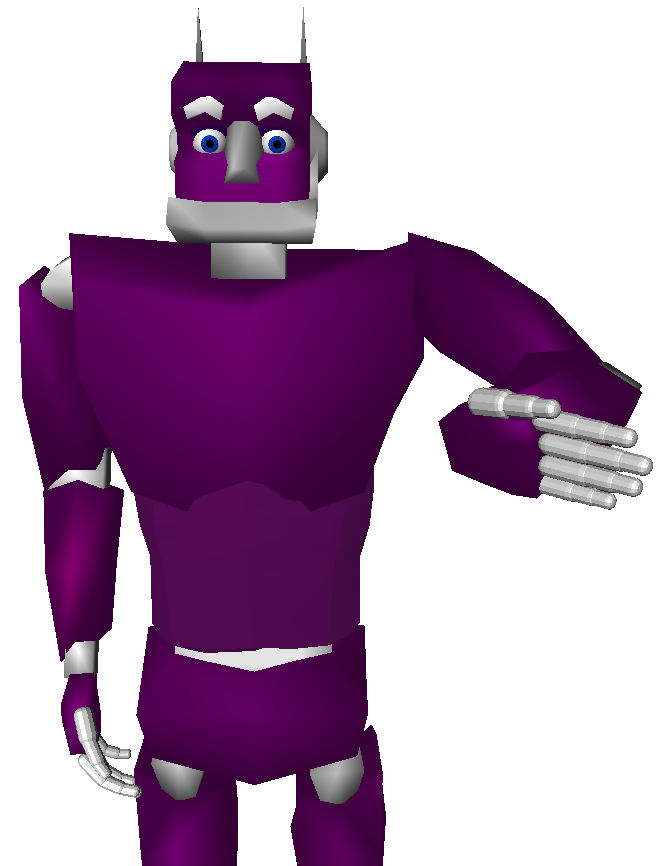
\includegraphics[scale=0.18]{./images/numack}
   \caption[Caption for NUMACK]{The Numack\protect\footnotemark  agent giving directions}
\end{figure}

\footnotetext{Image from http://www.articulab.justinecassell.com/projects/}

The different agents mentioned use diverse system for dialogue processing but in our case we will use narrative generation techniques so for the following part we will focus on the study of theses techniques and their applications.
\subsection{Interactive storytelling}
The standard approach to incorporating storytelling into a computer system is to script a story at design time and then have the story's script execute without variation at run-time. If a computer system uses a scripted story, its ability to adapt to the user's interactions is limited \citep{Riedl10}.\\

In educational and training applications, a limited number of stories or permutations of a single story, limits the ability of the system to adapt to a learner's needs. Interactive Storytelling is a branch of Artificial Intelligence that deals with narrative objects (literary, video-games, film) to understand, analyse or generate them by providing techniques that can be implemented by computer programs. For example, Narrative Generation techniques are designed to create multiple different scenarios from the same initial narrative data. Mostly based on planning techniques \citep{Young99}, the recent narrative generation systems can also fall under the logic programming area \citep{Bosser10}.
\subsubsection{Planning techniques}
The generation of narratives can be seen as a knowledge-based planning problem with associated issues concerning representation and real-time performance. Planning was initially proposed for Interactive Storytelling in \citep{Young99}, and since then it has emerged as the dominant technology for Interactive Storytelling prototype systems. A number of factors have contributed to this: one is the apparent natural fit between narratives and plans which enables narratives to be naturally modelled as a sequence of actions; another is that plans embed key features including causality among story events.\\

Hierarchical Task Network (HTN) planning \citep{Erol94} has been adapted to dynamically generate the character roles, by interleaving planning and execution, which supports dynamic interaction between actors, as well as user intervention in the unfolding plot \citep{Cavazza02}. This way, characters’ roles, rather than a centralised plot model, serve as the main driver for narrative generation. From a technical perspective these roles display an internal structure, which is also task-based, with an implicit level of intentions predicated on the story structure.\\

Throughout the narrative genres that have served to illustrate research in interactive narrative, there has been a prevalence of those genres based on actions and situations rather than the psychological relations between agents. One notable exception has been : Fa\c cade \citep{Mateas05}, a first-person, real-time, one-act interactive drama. It involved three major research efforts: designing ways to deconstruct a dramatic narrative into a hierarchy of story and behaviour pieces; engineering an AI system that responds to and integrates the player’s moment-by-moment interactions to reconstruct a real-time dramatic performance from those pieces; and understanding how to write an engaging, compelling story within this new organizational framework.\\

Another exception was FearNot! \citep{Aylett05}, a pedagogical system developed to address the question of bullying in schools. It uses emergent narrative and a cast of autonomous characters to create improvised bullying situations which are not predictable or completely controlled. The goal of this application is to enable children to explore bullying issues, and coping strategies, interacting with characters to which they become affectively engaged.\\

In his thesis, \citeauthor{Pizzi11} described a prototype in which characters’ behaviour is driven by a real-time heuristic search planner that applies operators whose content is based on a specific inventory of feelings.\\

After many years of using planning for narrative generation, research then concentrated on solving some remaining problems. \citeauthor{Porteous10} for example, suggested a solution to best control the shape of the narration generated and give a better support for real-time interactive performance. Their approach was to specify narrative control knowledge for a given story world using state trajectory constraints. Then to treat these state constraints as landmarks, using them to decompose narrative generation, in order to address scalability issues and the goal of real-time performance in larger story domains.\\

\citeauthor{Riedl10} described a solution to generate a sound and believable sequence of character actions that transforms an initial world state into a world state in which goal propositions hold. Their refinement search planning algorithm: Intent-based Partial Order Causal Link (IPOCL) planner, in addition to creating believable plot progression, reasons about character intentionality. It identifies possible character goals that explain their actions and creates plan structures that explain why those characters commit to their goals.\\

Even if planning has emerged as the dominant technology, featuring in a number of prototype systems, more recently, Linear Logic has been proposed as a suitable representational model for narratives because it supports causality \citep{Bosser10}. Masseron et al. \citep{Masseron93} have established how Linear Logic formalisation could support planning and how the properties of Linear Logic made it so that a proof in Linear Logic could be equated to a plan. It shows that Linear Logic is closely related to Planning but one of its advantages is that it has a standard semantics unlike Planning. 
\subsubsection{Linear logic programming}
\citeauthor{Dang13} provides a model, a method and a tool to produce interactive scenarios. The aim of his work is to assist the production of video games whose development meets the intentions of the authors while allowing a flow influenced by the player's choice (expressed by his/her actions). He models the scenario with linear logic and use its rigorous and automatic deduction mechanisms to control the flow of the game.\\

In their paper, \citeauthor{Martens13} explore the use of Linear Logic programming for story generation. They use the language Celf \citep{Schack08} to represent narrative knowledge, and its own querying mechanism to generate story instances, through a number of proof terms.\\

Celf programs are normally divided into two main parts: a \textit{signature}, which is a declaration of type and terms constants describing data and transitions, and \textit{query directives}, defining the problem for which Celf will try to find solutions.\\

Figure \ref{Figure celf} shows an example of Celf program representative of the form used to model narrative, and composed of signature and a query of 100 attempts to generate stories ending with the death of the character Emma (line 22). \\

The story elements available as well as the states of the story are the \textit{narrative resources} (lines 1-5). Transforming events occuring in the narrative (such as resource creation and consumption) are called \textit{narrative actions} (lines 6-14). The initial narratice environment is describes with the type init (line 15).\\

Once the narrative is modelled, it is run using Celf and the proof-terms obtained are post-processed for causality analysis using CelfToGraph. This program automatically transforms proof terms generated by Celf into directed acyclic graphs. Such graphs represent narrative plots, structured by narrative causality, where nodes are narrative actions and edges represent inferred causality relationships.\\

The major point of interest in this study was the variability of the stories generated. The code described allows to generate 72 different narrative sequences for 100 attempts. After an automatic comparison of the corresponding plots using CelfToGraph, they can exhibit 41 different plots, meaning that a number of different narrative sequences share the same causal structures. This allows the characterisation of classes of true story variants. \\

\begin{figure}[!h]
   	\centerline{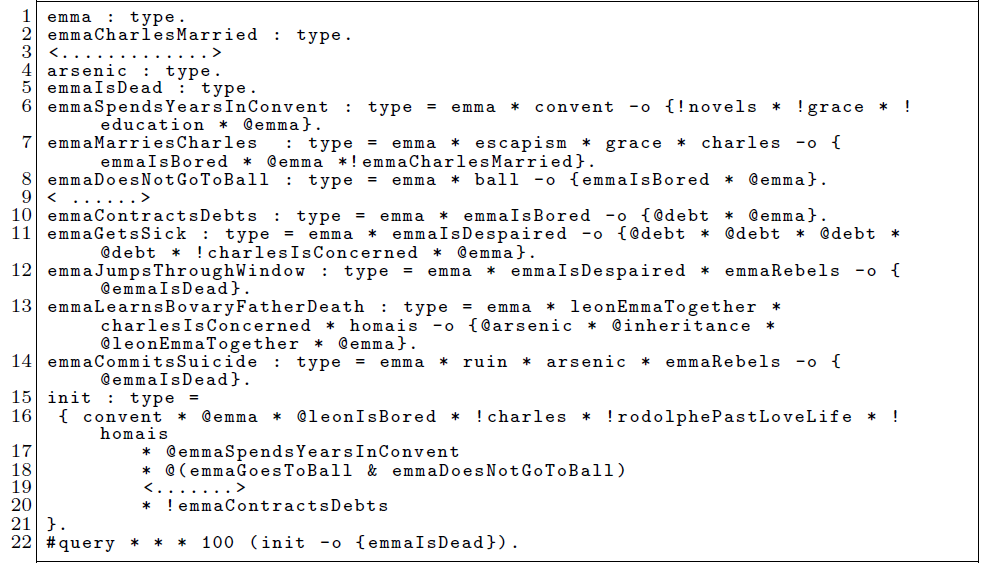
\includegraphics[scale=0.6]{./images/celf}}
   	\caption{\label{Figure celf} Example of the Celf program used \citep{Martens13}}
\end{figure}
\newpage
\subsection{Synthesis}
Most people with schizophrenia suffer from a strong social isolation due to the fact that they have difficulty communicating, even in the most mundane situations of daily life. Social skills training teaches the patients how to extend their behavioural repertoires in order to be able to communicate and regain some independence.\\

Serious games can be a great asset for social skills training as they provide a safe environment in which the patients can practice social interaction without the repercussions of emotional frustration and feeling of failure expected in the real world. The entertainment also increases their motivation and hold the patient's attention, which can increase the effectiveness of the training.\\

Embodied Conversational Agents (ECAs) have interesting properties for social skills training. For example they can generate verbal and non-verbal behaviours which is ideal for the training of facial expression recognition; skill that is usually altered in schizophrenia.\\

To adapt its answer and behaviour, the ECA can use different systems to detect the user's emotional state. This can be done using facial or vocal recognition, physiological signals via biosensors or psychological signals via electroencephalogram. For a better estimation of the user's emotional state, it is possible to combine these systems for a multi-modal approach. \\

It is particularly interesting from a therapeutic point of view, to be able to vary the scenarios of the game to lead patients to respond to unforeseen situations in a safe environment. Patients also need to train regularly but if they always do the same exercises they will lose interest and their training will not be efficient. Narrative generation is a solution to generate variations in a scenario and can be done using planning or linear logic techniques.
\newpage
\section{Contribution} \label{sec: Contribution}
\subsection{Research Question}
This internship combines the issues of interactive storytelling and serious games for therapeutic purposes. The problem raised by this project was : Could we find a narrative generation technique adapted to the underlying structure of the scenarios for social skills training that would obtain a sufficient level of variability for use in a therapeutic purpose? \\

The development of a prototype serious game using a game engine was initially the plan to answer to this question. We first imagined a game with a first-person perspective, where the game world would have been a town with shops, pharmacy and bank for example. The patient would have a task to do and in order to complete it he would have to move in the town and interact with the different elements available. But in order to be therapeutically valid, the scenarios of the game must be provided by specialist of the domain.\\

The primary task of the internship was to collect ideas of scenarios thought up by the psychiatric team of the CHU, that are to be used in session, to help patients with schizophrenia to behave appropriately in social situations of everyday life. We then had to analyse the structure of these scenarios and to identify the possible points of deviation in order to implement them in the form of an interactive game.\\

After further discussions with the psychiatric team, we found out that they were mainly using role playing activities based on self-affirmation exercises during their training sessions. The scenarios we were given had more of a dialogue structure rather than a succession of actions as we would expect in a traditional video game scenario. These sessions focus on the communications skills of the patients, for this reason the team pointed out the importance of the verbal and non-verbal contents of the dialogues. \\

The overall objective of the self-affirmation exercises is to extend the patients' behavioural repertoires by talking about different situations in an social context and by acting them out. For instance, these exercises can teach the patients how to : \begin{itemize}[noitemsep]
\item[-] introduce themselves
\item[-] start/maintain/interrupt a discussion
\item[-] request/refuse something
\item[-] receive/give a compliment
\item[-] receive/give a criticism
\end{itemize}
The team also explained that, in order for the patient to feel connected about the game, it would be better if the content of the dialogues are related to their personal life. The game RC2S \citep{Peyroux14} for example includes dialogues of a patient with his boss. This is not relevant with the patients that the team supervises because most of them are unemployed. If we want to talk about the family it is the same problem, most of them are single and don't have children so it is more relevant to talk about their parents, brothers and sisters, etc..\\

Based on our discussions with the team, we built a primary dialogue which will be use as a starting point for our project :  \\
\fbox{ \label{expl : Dialogue module 2}
\begin{minipage}{\dimexpr\linewidth-3\fboxrule-4\fboxsep}
Ami     : ``Salut \c{c}a va?" (joie)\\
Patient : ``Salut, \c{c}a va et toi?"\\
Ami     : ``Oui \c{c}a va" (joie)\\
Ami		: ``J'ai trouv\'{e} un travail, je commence lundi prochain!" (joie)\\
Ami		: ``Par contre ma voiture est en pane, j'ai besoin de la r\'{e}parer pour pouvoir y aller." (tristesse)\\
Ami		: ``Et mon curateur ne veut pas me donner d'argent pour faire les r\'{e}parations." (tristesse)\\
Patient	: ``C'est super que tu aies trouv\'{e} du travail!"\\
Ami		: ``Oui mais sans voiture je ne pourrais pas y aller." (col\`{e}re)\\
Ami		: ``Tu ne pourrais pas me pr\^{e}ter de l'argent pour faire les r\'{e}parations?" (joie)\\
Patient	: ``J'aurais aim\'{e} pouvoir t'aider mais je n'ai pas d'argent."\\
Ami		: ``Ah, ok. Il va falloir que je trouve une solution." (neutre)\\
Patient	: ``Tes parents ne peuvent pas t'aider?"\\
Ami		: ``Je n'ose plus leur demander de l'aide, \`{a} chaque fois je vois bien que ça les emb\^{e}te." (tristesse)\\
Patient	: ``Mais cette fois si c'est pour aller au travail peut-\^{e}tre qu'ils seraient contents de t'aider."\\
Ami		: ``Oui, peut-\^{e}tre. Je les appellerais ce soir pour voir." (neutre)
\end{minipage}
}\\[2.5ex]

Although the dialogue is now in place, the scientific question becomes : \textbf{Can we find a narrative generation technique adapted to the underlying structure of \emph{dialogues} that would obtain a sufficient level of variability for use in a therapeutic purpose?} \\

Having already made the choice to use a narrative generation technique using linear logic (LL), this question becomes much more challenging than the previous one. The generation of a dialogues having cognitive properties with LL has never been attempted in the past. We have reasons to believe that it is possible : the English prototype for the Companions project \citep{Smith11} for instance, uses narrative generation technique based on planning to perform an appraisal of the affective situation and then select appropriate communicative acts that construct a narrative response. An approach using LL to build and validate plans for dialogues between agents in a Multi-Agents System has been suggested in \citep{Dixon09}. This solution is designed for task-related discussions between two agents and is not adapted for the generation of emotionally charged dialogues in an interactive context.\\ 

To answer this problem we will prototype a serious game using an Embodied Conversation Agent (ECA) with whom the patients can interact. The ECA must have some properties such as being able to generate facial expressions, in order to train the patient to recognise them. Due to the patient's inability to express emotions effectively and their lack of awareness of this problem \citep{Peyroux14,Weiss09}, it would be an advantage if the ECA read their emotions and changed its behaviour accordingly.
\subsection{Proposition}
%TODO : explain why 
The following is a list of the elements which needed to be considered in our solution to the problem. All these elements are described in more detail in the next section.
\begin{itemize}[noitemsep]
\item A dialogue modelled using linear logic (LL) formalism which allow variations. The dialogue is structured in terms of resources and actions and includes the emotions of the ECA and the patient.
\item The adaptation of the facial emotion recognition program so it fits our case of study.
\item The implementation of new commands in the tool that we chose to explore the use of linear logic applied to narrative generation and story telling. These new commands make it possible to use this tool into an interactive application.
\item We also added in this tool the possibility to ``Go back in time". This allow the patient to undo his last actions and see what would happen if he did another choice, which is very interesting in a therapeutic point of view.
\item A prototype serious game composed of 3 modules :
\begin{itemize}
\item Module 1 is used to train the patient to recognize facial expressions on the ECA.
\item Module 2 has the same purpose as Module 1 but this time the ECA speaks which put the emotions into a context.
\item Module 3 is the most important module. In this module the patient can maintain a conversation with the ECA. A list of answers is suggested to the patient and the dialogue progress depending on his choice and his facial expressions.
\end{itemize}
\end{itemize}
\subsection{System description}
In order to give a solution to the problem, we developed a serious game using an ECA. This application has been built in the language C\# using Visual Studio and the graphical class library Windows Forms which is included as a part of Microsoft .NET Framework. It provides a platform to write client applications but does not offer a comparable Model-View-Controller (MVC) paradigm. \\

The program uses a collection of systems :
\begin{enumerate}
\item In order to offer an ECA with whom the patients can interact, we needed a system that would provide us with characters and would allow us to animate them in real-time. We decided to use HapFACS\footnote{http://ascl.cis.fiu.edu/hapfacs-open-source-softwareapi-download.html}, a program developed by one of our partner: the University FIU of Miami.
\item For the generation of the dialogues, we needed a system using narrative generation techniques and which was usable in an interactive application. We could have used the language Celf \citep{Schack08} presented in the section \ref{sec: State of the art}.3.2 but as we needed to define an ad-hoc interaction paradigm, we decided to use TeLLer\footnote{Project TeLLer. Page maintained by Jo\~{a}o F. Ferreira (University of Teesside) gathering programs to test the use of linear logic for computational narrative. https://github.com/jff/TeLLer.}, a program designed by Jo\~{a}o F. Ferreira from Teesside University.
\item Knowing that a lot of patients have issues with expressing their own emotions, the psychiatric team suggested that it would be interesting if the ECA adapts its behaviour to the patient's facial expressions. In order to respect the patient's medical confidentiality we had to find an off-line system for the facial emotion recognition. This criteria is very restrictive and the only solution that we found was the Intel\textsuperscript{\textregistered} Perceptual Computing SDK\footnote{https://software.intel.com/en-us/perceptual-computing-sdk}.
\end{enumerate}
 
The structure of the application can be represented as in the diagram Figure \ref{Figure diagram module 3}.\\
The application is multi-threaded, the main thread is used to display the window and another thread is needed for the emotion recognition system. To communicate with the program TeLLer we use a \emph{Process} component that allows us to start a process and provides access to it while it's running. With this component we can write on the standard input and read the standard output of TeLLer. As we have been provided the code of HapFACS, we integrated it into our application which will facilitate its use. Each system used in the program will now be described in details.
\begin{figure}[!ht]
   	\centerline{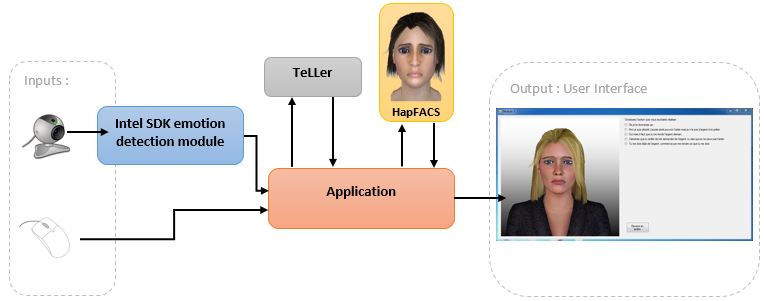
\includegraphics[scale=0.9]{./images/module3_diagram}}
   	\caption{\label{Figure diagram module 3} System architecture}
\end{figure}

\subsubsection{Detection of the emotion expressed by the patient}
As mentioned earlier, patients often have issues with expressing their own emotions and are not aware of these issues \citep{Weiss09, Peyroux14}. This can cause them to be misunderstood by people having a conversation with them. We can easily imagine a scenario where a patient is informed of some positive news that really makes him happy. But when he speaks of his delight, his incapability of expressing his emotions can make him seem sarcastic. \\

Therefore it is a useful exercise to place the patients into this kind of situation where the expressed emotion provokes a feedback from the ECA. It has been suggested by the psychiatric team that it could teach them how to react appropriately as well as to make them aware of their deficit. \\

For the facial emotion recognition system we used the Intel\textsuperscript{\textregistered} Perceptual Computing SDK which is a library of pattern detection and recognition algorithm implementations exposed through standardized interfaces. The SDK emotion detection module estimates facial emotion states from image sequences which can be provided by the web-cam. \\

With the psychiatric team we decided to simplify the problem by reducing the list of Ekman's universal emotions \citep{Ekman77} to only 3 elements : happy, sad and angry to which we added neutral. This restricted set has been proved efficient in the past as it has been chosen in the the program Ga\"{i}a \citep{Gaudelus12} (described in section \ref{sec: State of the art}). \\

We modified one of the sample that comes with the SDK which is a GUI application to demonstrate emotion detection capabilities. The code provided returns an enumeration of \emph{EmotionData} that itemizes the supported emotion states. This list contains the following emotions : anger, content, disgust, fear, joy, sadness and surprise. We restricted this enumeration to the set of emotions retained in our case of study.\\

The \emph{EmotionData} is a structure that describes the parameters of a detected emotion. Only one of these parameters is used in our case : the \emph{intensity}. To determine the emotional state of the patient we sort the emotions by their intensity and the highest one is selected. If the intensity is under a certain level, the emotion of the user is defined as neutral. We now know the emotional state of the patient recognised by the system. This value is updated every 500 milliseconds to ensure us to have a correct estimation when the patient interact with the system.

\subsubsection{TeLLer}
From a therapeutic point of view, it is particularly interesting to be able to vary the dialogues of the game to lead patients to respond to unforeseen situations in a safe environment. Patients also need to train regularly but if they always do the same exercises they will lose interest and their training will not be efficient. \\

Narrative generation is a solution to generate scenarios and in our case, to generate dialogues. TeLLer is a tool that explore the use of Linear Logic for narrative generation. It generates stories based on knowledge provided to the system via a file containing code such as in Annexe \ref{annexe: Code TeLLer}. In this section I will explain how I built the dialogue using Linear Logic and how we had to implement new commands in TeLLer in order to allow the patient to interact.\\

The interaction paradigm for this application is quite simple. It's a turn-by-turn dialogue between the ECA and the patient. Once the ECA finished its sentence, the patient is offered a list of choices in which he can choose a response. His facial expression is also taken into account as part of his interaction. Unlike in the Companions project \citep{Smith11}, it is not possible to interrupt the ECA while it's talking. This is due to the fact the the speech acts are atomic in TeLLer, therefore they can not be fragmented.\\ 

To model the dialogue in our application, we used a fragment of linear logic with the following connectors:\\
$\multimap$ : Linear implication (-@ in TeLLer's syntax). The resources on the left-hand side are consumed to produce the resources present on the right-hand side. Example: ``1 euro $\multimap$ 500g of strawberry" means that we must give 1 euro to get 500g of strawberries.\\
$\otimes$ : Multiplicative conjunction (* in TeLLer's syntax). Expresses the joint presence of elements. Example: ``1 euro $\multimap$ 500g strawberries $\otimes$ 500g tomatoes" means that by giving 1 euro we can buy 500g of strawberries and tomatoes. \\

The left-hand side of the sequent contains the description of the initial conditions, considered as resources to use up while unfolding the dialogue. We considered the narrative environment as a representation of the ``ECA's mind". The resources available in the environment thus include emotional state of the patient, subjects of discussion available and the various states of the discussion. A sample of code is available in annexe \ref{annexe: Code TeLLer}.\\

One of the most difficult task when implementing the dialogue was to build a discussion that made sense. The consistency is kept by dividing the dialogue into a collection of subjects, each of them represented by a resource. When the ECA starts to talk about a subject, it consumes the resource corresponding and produces transitional resource. When the end of the subject is reached, the last transitional resource is consumed and a new resource is produced, informing the ECA that it can pick a new subject in the available ones.\\

With this structure of dialogue, the different topics of discussion are competitive, this produce the variability. But inside a subject, the discussion is scripted which is a break for the variability of the dialogue. We are currently working on a solution that would allow interactions between the different subjects but by lack of time we can not suggest a working solution in this report. \\

Here is a sample of code illustrating the structure of the dialogue :
\begin{lstlisting}[basicstyle=\small]
greet * newJob * lottery
greet -@ A "agent / Salut, ça va ? / aHappy"
A -@ B "patient / Ca va et toi ?"
A -@ C "patient / Ca ne va pas super bien"
B * pHappy   -@ subjectDone "agent / Oui ça va. / aHappy" 
B * pNeutral -@ subjectDone "agent / Oui ça va. / aHappy" 
B * pSad     -@ E "agent / Tu es sûr ? Ca n'a pas l'air d'aller. / aNeutral"
B * pAngry   -@ E "agent / Tu es sûr ? Ca n'a pas l'air d'aller. / aNeutral"
[...]
subjectDone * newJob -@ K "agent / J'ai trouvé un nouveau travail ! / aHappy"
subjectDone * lottery -@ P "agent / J'ai gagné 50 euros au Banco hier ! / aHappy"
[...]
\end{lstlisting}
The first line enumerates the available resources in the environment at the beginning of the discussion. When the game starts the only feasible action is the consumption of \textit{greet} and production of \textit{A}. Once the greeting is done, the resource \textit{subjectDone} is produced allowing the ECA to pick a new subject between \textit{newJob} and \textit{lottery}.\\

When the same resources are on the left-hand side of two (or more) sequent (resource A in the example), it generates a choice point. This means that in order for the dialogue to continue, someone (the ECA or the patient) has to make a choice within the possibilities. In the code above, the consumption of the resource \textit{A} offers two choices : the production of \textit{B} or \textit{C}. We had to find a solution that would allow the system to know if the choice point is addressed to the ECA or the patient. This is done using the the possibility in TeLLer to name actions using speech marks.\\

We named all the actions of the dialogue in a specific way : ``actor / sentence said / and emotion to express if the actor is the ECA". Thanks to this naming, the system instantly know who needs to choose an action. If the actor is the patient, then all the possible choices are displayed as illustrated in Figure \ref{Figure module 3}.\\

When the patient gives a response, his facial expression is evaluated by the facial emotion recognition system. This estimation is added to the environment allowing the system to adapt its answer. If the expression of the patient does not correspond to his felt emotions the system may react inappropriately resulting in the misunderstanding from the patient.\\

Unfortunately we had initially no way of adding/deleting resources with TeLLer once the game was running. It was only possible to use these commands before to start the game. To allow the ECA to adapt its answer, we need to update regularly the perceived emotion of the patient in the environment. For this reason we had to change the implementation of the \textit{+} and \textit{-} commands in TeLLer in order to be able to use them at any time during the game. This way, we can delete the previous expression and add the new one in the environment.\\

In a therapeutic point of view, it is very interesting to be able to offer the patient the possibility to undo his previous actions and try different ones. This way he can try new behaviours and see what would happen if he did something else. If he does not understand one of the ECA's answer, he can replay the action as many times as he wants.\\

To allow this possibility we had to implement new commands in TeLLer.\\
The first one is the \textit{choicepoints} command that returns the list of all the choice points previously encountered. Thanks to this list we can build the user interface (see Figure \ref{Figure backintime}) that can be used by the patient to undo his actions and ``go back in time".\\
This is an example of list returned :
\begin{lstlisting}[basicstyle=\small]
[(1,"action 2", ["choice 2", "choice 3"])(0,"action 1",["choice 0", "choice 1"])]
\end{lstlisting}
It contains two choice points which are listed in reverse chronological order (the first one in the list the one that occurred last). Each choice point in the list is represented between brackets and contains an index, the name of the last action that occurred, and the list of all the choices that were possible. We use these two last elements to build the user interface. The index with is used with the command \textit{goto} that allows the user to go back to the desired choice point and to start again the dialogue. \\

This option can be a useful tool when the patient debrief his training with a member of the psychiatric team. Together, they can replay the game and try different behaviour and with the comments of the clinician the patient can have a better understanding of his actions.						

\subsubsection{HapFACS}
For the animation of the ECA we used HapFACS \citep{Amini13}, an open-source software and API developed by the University FIU of Miami (see Figure \ref{Figure hapfacs API}). It uses the Haptek Player\footnote{http://www.haptek.com} and characters created in the commercial software PeoplePutty\footnote{http://www.haptek.com/products/peopleputty/} from the Haptek company.\\
\begin{figure}[!h]
   	\centerline{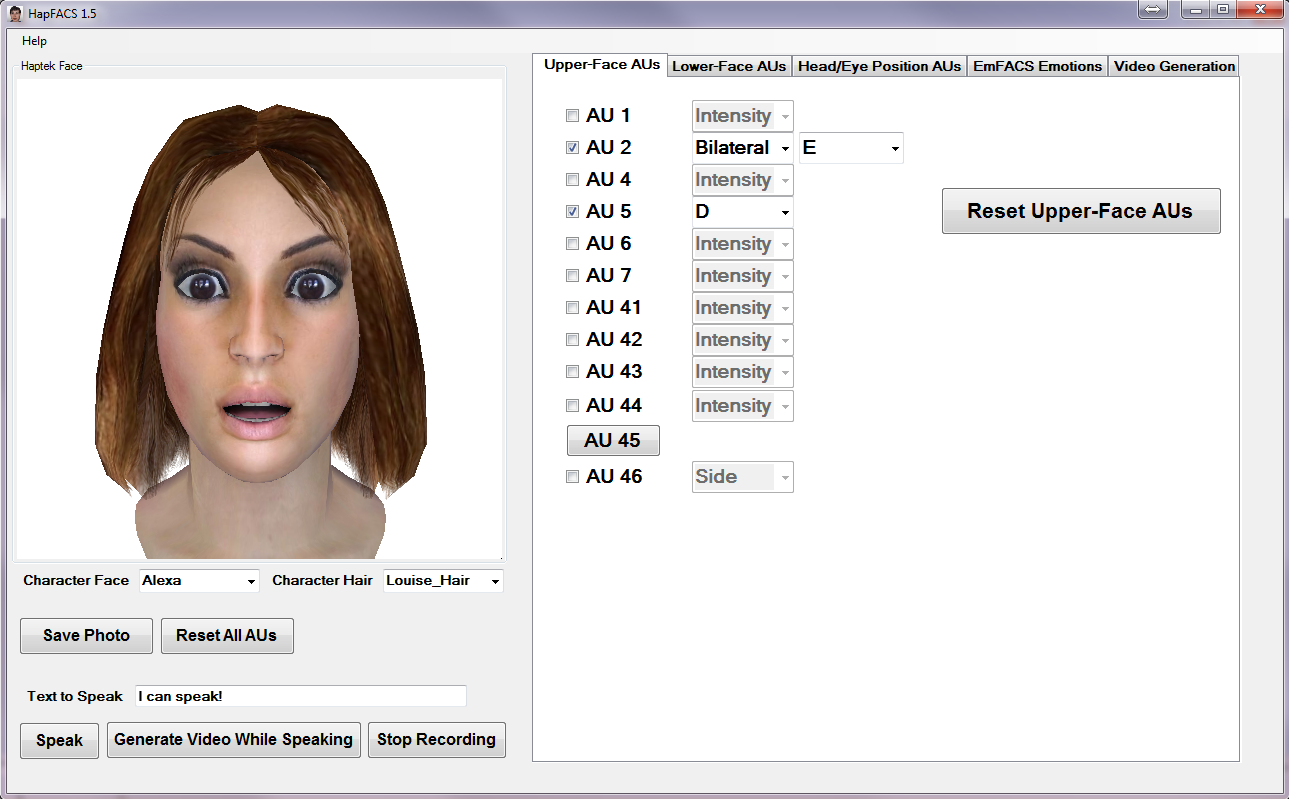
\includegraphics[scale=0.4]{./images/hapfacsAPI}}
   	\caption{\label{Figure hapfacs API} HapFACS interface for generating static outputs of AUs. \citep{Amini13}}
\end{figure}

The Haptek software is an avatar system widely used in research projects over the years \citep{Smith11, Fellner12, Lisetti13}. This system can be easily integrated to applications and provide a real-time talking character with lip synchronisation. However, the lack of an accessible programming interface allowing the generation of facial expression complicates its use in other applications. The HapFACS software addresses this issue by providing an API to control facial expressions in real-time based on the FACS and . \\

The HapFACS system also allows the control of emotions based on the Emotional FACS (EmFACS) \citep{Friesen83} which provides subsets of AUs in FACS that are relevant to facial expressions of the universal emotions identified by Ekman \citep{Ekman77}. This is exactly what we needed to animate our ECA. By using this system, we don't have to work out what specific AUs or points we need to move on the ECA's face to generate an expression because HapFACS provides us with a range of functions (such as Happiness(intensity), Sadness(intensity), etc.) which are very easy to use. \\

The animation of the ECA during the discussion is very easy. As we explained earlier, the name of the actions for the ECA is structured as follows : ``agent / sentence said / ECA's emotion". This naming provides all the required informations to animate the ECA : the text to say and the emotion to express. \\
\subsection{Running example}
The application is compatible with Windows 7, in order to start the game we just have to launch the executable file. This will open a Menu window that contains three buttons, each of them leading to a different Module of the training session. \\

Each Module starts with a little introduction explaining the rules of the game (see Figure \ref{Figure consignes}) and finishes with a message of thanks and a navigation button to go back to the Menu.
\subsubsection{Modules 1 and 2}
The only purposes of these modules are to train the patient in the recognition of facial expression and to familiarize him with the system. \\

In the first module (see Figure \ref{Figure module 1 and 2}), the ECA only expresses different facial expressions with three level of intensity each. The patient has to identify the emotion, select his answer from the list provided and validate it. An instant feedback is shown indicating if the answer was correct. \\

In the second module, a conversation is simulated between the ECA and a second participant whose input is shown to the patient as text. The dialogue described in section \ref{expl : Dialogue module 2} is used for this conversation. The patient's task is exactly the same as in the first module. The only difference is that by simulating a conversation, the facial expressions are put into a context and according to \citep{Lee13}, ``schizophrenic patients are capable of benefiting from situational context when evaluating ambiguous emotional expressions of faces".
\subsubsection{Module 3}
This module is the one that has to be considered as the proposed answer to the problem. It uses all the systems described in section 3.3 (unlike the two previous modules) allowing the generation of the dialogue and its variation depending on the patient's interactions. \\

The module 3 starts with the ECA smiling and asking the patient how he feels (``Salut \c{c}a va?"). The patient is offered two choices of answers : ``\c{C}a va et toi ?" or ``\c{C}a ne va pas super bien". If the patient choose the first answer and the emotion recognition system detects that he has a sad emotion, the ECA will then ask ``Tu es s\^{u}r? \c{C}a n'a pas l'air d'aller". On the other hand, if the system detects that the patient has a happy emotion, it will continue the discussion with one of the available subjects.\\

The figure \ref{Figure module 3} contains an example of the ECA asking for money to fix its car. As we explained in section 3.1, we used self-affirmation exercises to build the dialogues. Here is a concrete example where the target for the patient is to refuse to help. In the list of answers suggested, each one represent a different behaviour studied during these exercises. \\
- ``Ok je te donnerais \c{c}a" this answer is for people who feel obliged to say Yes even when they would like to say No.\\
- ``Non je suis d\'{e}sol\'{e}, j'aurais aim\'{e} pouvoir t'aider mais je n'ai pas d'argent \`{a} te pr\^{e}ter." this is a correct way to express a refusal, using empathy, saying 'I' and being specific.\\
- ``Oui mais il faut que tu me rende l'argent demain" this answer is for people who can't say No at once, and prefer to say Yes But ... and then ask something impossible to do like in this case, give the money back the day after.\\
- ``Tu me dois d\'{e}j\`{a} de l'argent, commence par me rendre ce que tu me dois". this is an aggressive behaviour that is likely to end up in an argument.\\
- ``J'aimerais que tu arr\^{e}te de me demander de l'argent, tu sais que je ne peux pas t'aider." this answer is more complex, it can be aggressive or empathic depending on the facial expression of the patient. The answer of the ECA will be different for each answer selected and facial expression of the patient.\\

If the patient realises that he made a mistake or if he is curious to see what would have happen if he selected a different action, he has the ability to go back in time by clicking the button ``Revenir en arri\`{e}re" (see Figure \ref{Figure module 3}). This will open a window listing the stages where the patient could interact and summarizing the possible answers as shown in the Figure \ref{Figure backintime}. \\

By clicking one of the boxes, the game will go back to the desired state and the patient can play again. This is interesting in a therapeutic point of view because it allows the patient to try different behaviour and see what is the best one to adopt.
\clearpage
\begin{figure}
   	\centerline{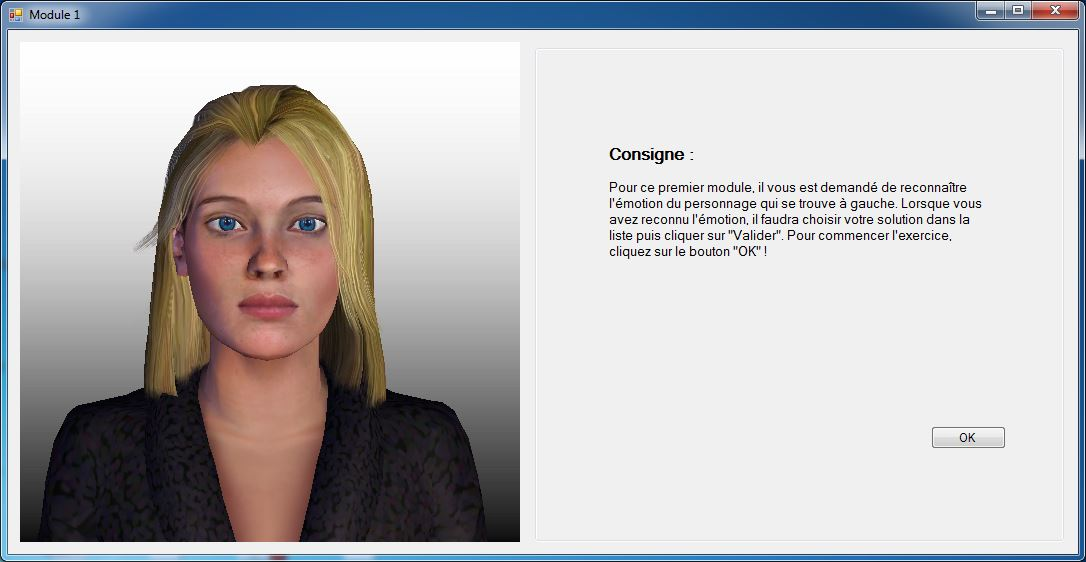
\includegraphics[scale=0.61]{./images/consignes}}
   	\caption{\label{Figure consignes} Explications for the Module 1}
\end{figure}
\begin{figure}
   	\centerline{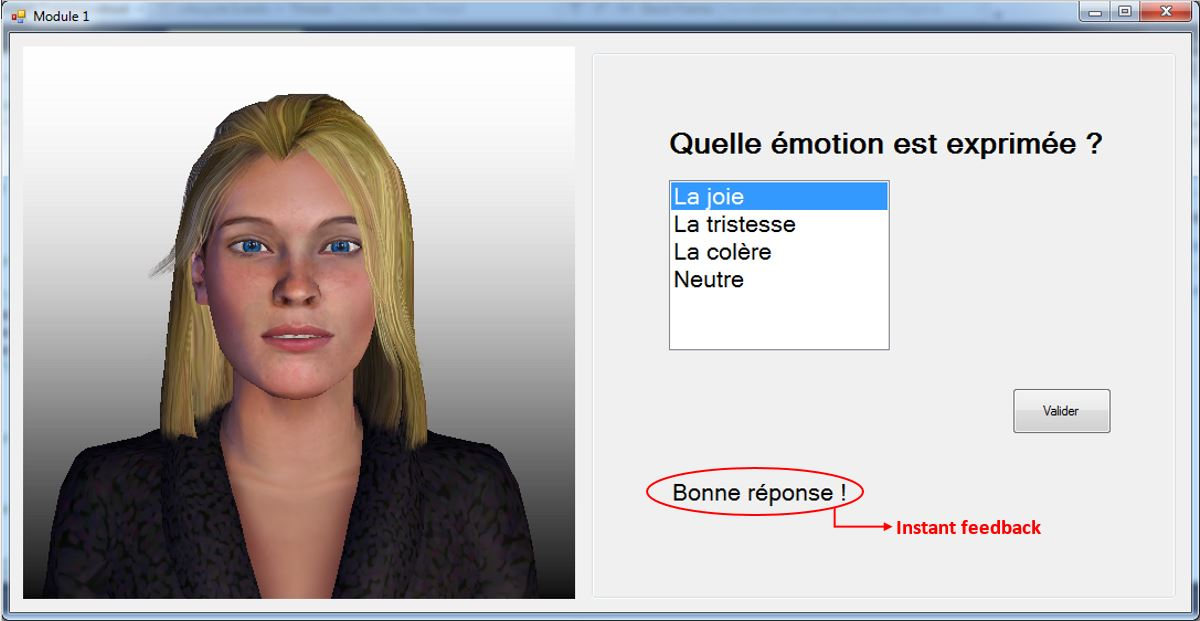
\includegraphics[scale=0.55]{./images/module1&2}}
   	\caption{\label{Figure module 1 and 2} User interface for the Modules 1 and 2}
\end{figure}
\begin{figure}
   	\centerline{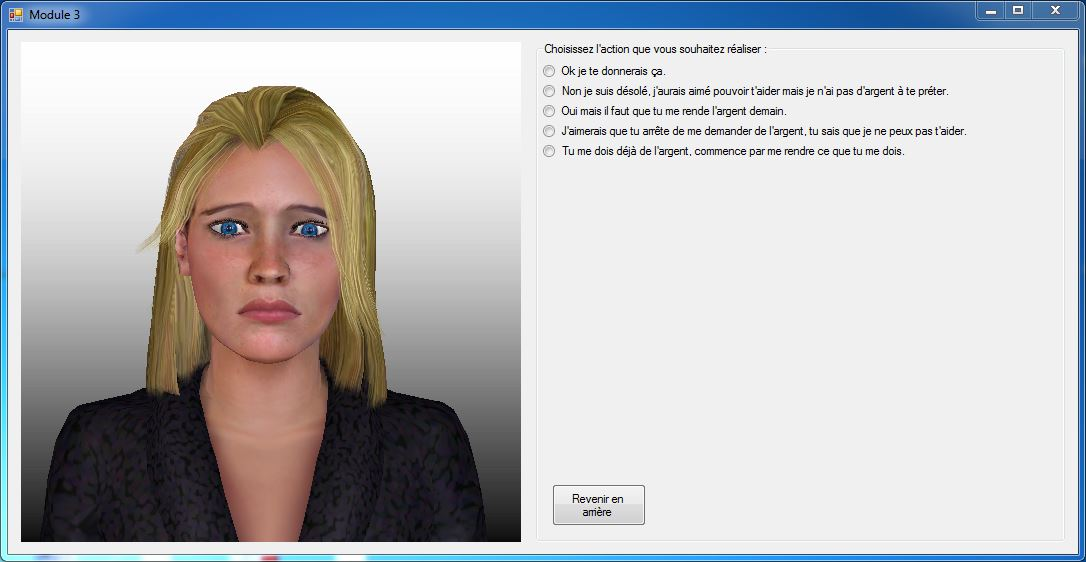
\includegraphics[scale=0.61]{./images/module3_general}}
   	\caption{\label{Figure module 3} User interface for the Module 3}
\end{figure}
\begin{figure}
   	\centerline{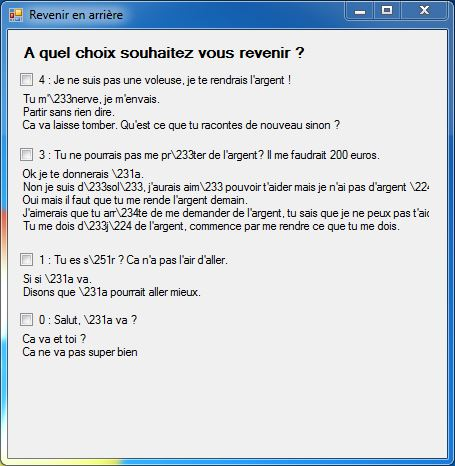
\includegraphics[scale=0.75]{./images/module3_backintime}}
   	\caption{\label{Figure backintime} Interface for the "Go back in time" option}
\end{figure}
%*****************************************************************%
\clearpage
\section{Evaluations} \label{sec: Evaluations}
\subparagraph{Technical evaluation}\mbox{}\\
A technical evaluation is planned to evaluate the level of variability of the dialogue generated by the system. We will use a functionality of TeLLer that allows the analyse of the generated stories. 
\subparagraph{Acceptance evaluation}\mbox{}\\
We will also evaluate the acceptability of the system from the patients. This evaluation will be set up and conduct by the the psychiatric team.
\subparagraph{Performance evaluation}\mbox{}\\
If the system is accepted by the patients, we will evaluate its performance. It has been mentioned by the psychiatric team that the modules 1 and 2 could eventually be used to see the progress of the patient after completing the training. The idea was to evaluate their ability to recognise facial expressions before the first session and after 6 months of training for example, and to see if they had made any progress.\\
The problem with this kind of evaluation is that it only focus on the recognition of facial expression without a context. Although, the studies conducted by \citeauthor{Lee13} demonstrated the importance of the situational context when recognising facial expression.\\
The development of a protocol adapted for the evaluation of the performance of this system would need a separate study that we can not conduct during this internship. This study should be conducted by specialists.\mbox{}\\

However, we can not describe the experimental protocol that will be used for the technical and the acceptance evaluations because they are not established yet. We are currently working on it and should be able to start the experiments before the end of the internship. \\
\newpage
\section{Synthesis and future work}\label{sec: Conclusion and future work}
During this internship we tackled the problem of finding a narrative generation technique adapted to the underlying structure of dialogues, that could be use in a serious game for patients suffering from schizophrenia in order to provide social skills training. \\

This problem is actually made up of three key elements : the generation of dialogue providing a high level of variability; the use of these dialogues by an ECA allowing social interactions; and finally, the use of this ECA in a cognitive remediation program to improve social skills of schizophrenic patients.\\

To address this problem we used TeLLer, a program that explores the use of linear logic applied to narrative generation and story telling. In order to use this program for the generation of dialogue, we had to find a way of representing a dialogue with resources. The dialogue generated has to provide the ECA with a speech and an emotion to express and has to vary depending on the actions of the patient and his facial expression. \\

In this report we propose a method of modelling a dialogue that meets all these criteria. In fact, the variability is generated by the variation of the subject of discussions. But inside a subject, the dialogue is scripted. We are currently working on a solution that would provide a higher level of variability by allowing concurrency inside these subjects. \\

To demonstrate the usability of our solution we prototyped an application for social skills training which contains three modules. The first two modules are used to train the patient in emotion recognition. They only differ by the fact that in the second module, the emotion is placed into a context which usually facilitates its recognition \citep{Lee13}. The third module uses our proposition and offers an agent with verbal and non-verbal behaviour to the patient with whom he can interact.\\

We are planning on adding modules where the level of difficulty would be gradually increased. We are currently trying to introduce ambiguity in the dialogue using sarcasm for example. In these kind of situation, only a correct recognition of the facial expression can unlock the situation.  \\

In the near future we want to improve the transition of the ECA's facial expressions. Currently, it changes abruptly from one to another but in order to increase the ECA's believability we need to make the transitions more fluid.\\

Another element of the ECA's facial expression that requires attention is its duration. For the moment, it lasts as long as the character's sentence, but it is known that the duration of the expression is highly variable \citep{Verduyn09}. \\

At present, the emotion of the ECA is part of the action, but it could be interesting to specify an emotional model that would control the emotion independently, which could produce even more variability into the dialogues.


%*****************************************************************%
\newpage
%\bibliographystyle{abbrv}
\bibliographystyle{apalike}
\bibliography{ref}

\newpage
\appendix
\section{Sample of code for the implementation of the dialogue using Linear Logic for TeLLer} \label{annexe: Code TeLLer}
\begin{lstlisting}[basicstyle=\small]
greet * newJob * pbcar * pbmoney * lottery

greet -@ A "agent / Salut, ça va ? / aHappy"

A -@ B "patient / Ca va et toi ?"
A -@ C "patient / Ca ne va pas super bien"

B * pHappy   -@ subjectDone "agent / Oui ça va. / aHappy" 
B * pNeutral -@ subjectDone "agent / Oui ça va. / aHappy" 
B * pSad     -@ E "agent / Tu es sûr ? Ca n'a pas l'air d'aller. / aNeutral"
B * pAngry   -@ E "agent / Tu es sûr ? Ca n'a pas l'air d'aller. / aNeutral"

C * pHappy   -@ F "agent / Ca à l'air d'aller pourtant / aHappy"
C * pSad     -@ G "agent / Oh moi nonplus ça ne va pas. / aSad"
C * pNeutral -@ G "agent / Oh moi nonplus ça ne va pas. / aSad"
C * pAngry   -@ G "agent / Oh moi nonplus ça ne va pas. / aSad"

E -@ subjectDone "patient / Si si ça va." 
E -@ I "patient / Disons que ça pourrait aller mieux."

I -@ G "agent / Oh moi nonplus ça ne va pas. / aSad"

F -@ J1 "patient / Pourquoi tu dis ca ?"
J1 -@ subjectDone "agent / Parce que tu as l'air joyeux. / aHappy"
F -@ J2 "patient / Non ca ne va vraiment pas."
J2 -@ G "agent / Oh moi nonplus ça ne va pas. / aSad"

subjectDone * newJob -@ K "agent / J'ai trouvé un nouveau travail ! / aHappy"
G * pbcar -@ L "agent / J'ai un problème avec ma voiture, elle a besoin de réparations. / aSad"
K * pbcar -@ L "agent / J'ai un problème avec ma voiture, elle a besoin de réparations. / aSad"
G * pbmoney -@ M "agent / Mon curateur ne veut pas me donner d'argent. / aAngry"
L * pbmoney -@ M "agent / Mon curateur ne veut pas me donner d'argent. / aAngry"
M -@ N "agent / Tu ne pourrais pas me préter de l'argent? Il me faudrait 200 euros. / aSad"

N -@ Nyes "patient / Ok je te donnerais ça."

Nyes * pAngry -@ O "agent / Tu es sur? Ca a l'air de t'énerver. / aNeutral"
Nyes * pSad -@ O "agent / Tu es sur? Ca a l'air de t'embéter. / aSad"
Nyes * pHappy -@ subjectDone "agent / Oh merci ça va beaucoup m'aider / aHappy"
Nyes * pNeutral -@ subjectDone "agent / Oh merci ça va beaucoup m'aider / aHappy"
[...]
\end{lstlisting}
\end{document}

%TODO : sarcasm ?